%%%%%%%%%%%%%%%%%%%%%%%%%%%%%%%%%%%%%%%%%%%%%%%%%%%%%%%%%%%%%%%
\section{PD Design}
\label{sec:fdsp-pd-design}
%\metainfo{(Length: TDR=50 pages, TP=20 pages)}
%\metainfo{\color{blue} Content: Conveners}

\fixme{Include an image of the subsystem, indicating its parts. Show how the system fits into the overall system).}

At the time of the Technical Proposal there are three photon collector options  under consideration, 
in the following we summarize the design and development status for each. 
[For the Technical Design Report there will be a baseline design and an alternate.]

%%%%%%%%%%%%%%%%%%%%%%%%%%%%%%%%%%%
%\subsection{Photon Collector}
%\label{sec:fdsp-pd-pc}
%\metainfo{\color{blue} Content: Cavanna/Whittington/Machado}


\subsection{\color{red}\bf Photon Collector: Dip-Coated Light Guides (4 pages)}
\label{ssec:fdsp-pd-pc-bar1}
\metainfo{\color{red} \bf Content needed: Toups}

\subsection{Photon Collector: Double-Shift Light Guides}
\label{ssec:fdsp-pd-pc-bar2}
%\todo{\color{blue} Content: Whittington}

The double-shift light guide photon collector design aims to maximize the active VUV-sensitive 
area of the photon detection system module while minimizing the necessary photocathode (SiPM) 
coverage. 
Commercially-fabricated plastic can be manufactured to transport light via total internal 
reflection with low attenuation losses. However, direct application of coatings to such
 manufactured optical surfaces can have an adverse impact on the effective attenuation length 
by introducing or exaggerating imperfections in the surface quality. 
To maintain the long intrinsic attenuation length of a manufactured light guide, the 
double-shift light guide design decouples the conversion of VUV photons to optical by
 arraying acrylic plates coated with TPB in front of a commercially-fabricated polystyrene 
light guide doped with a second wavelength-shifting compound.

\paragraph*{Description}

Figure~\ref{fig:DoubleShiftLG-Cartoon} illustrates the process by which LAr scintillation 
photons are converted and detected by a double-shift light guide module. VUV scintillation
 photons impinging on the acrylic plates are converted to blue wavelengths. A portion of
 these blue photons penetrate the light guide and are converted to green. The isotropic 
re-emission of these green photons leads to a significant fraction becoming trapped by 
total internal reflection within the light guide. Trapped photons are transported to 
the end of the light guide where they are detected by an array of SiPMs.

%\begin{figure}[ht]
%  \begin{center}
%  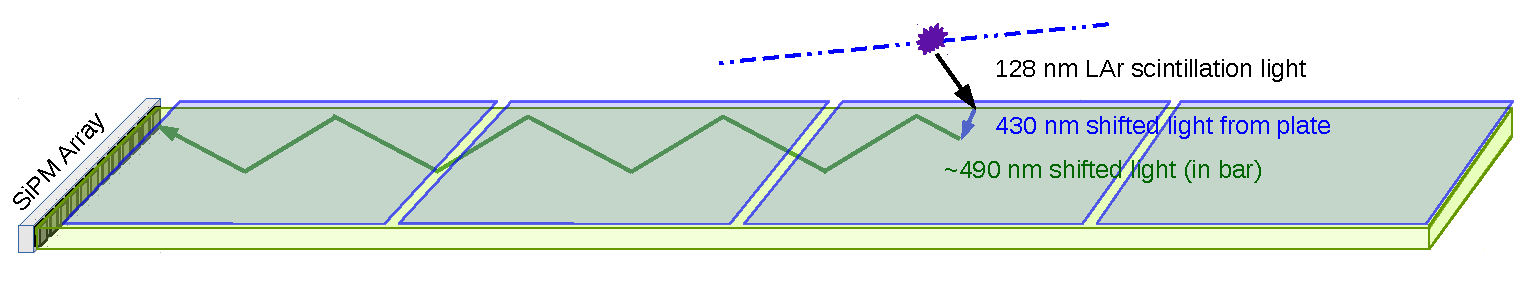
\includegraphics[width=0.9\columnwidth]{pds-DoubleShiftLG-Cartoon.pdf}
%  \caption{Cartoon schematic of the operation of a double-shift light guide.}\label{fig:DoubleShiftLG-Cartoon}
 % \end{center}
%\end{figure}

\begin{dunefigure}[Cartoon schematic of the operation of a double-shift light guide.]{fig:DoubleShiftLG-Cartoon}
{Cartoon schematic of the operation of a double-shift light guide.}
  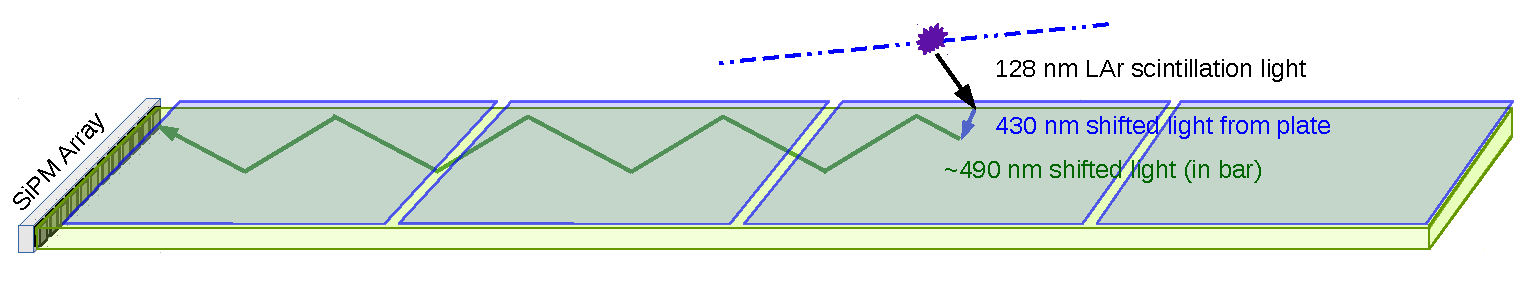
\includegraphics[width=0.9\columnwidth]{pds-DoubleShiftLG-Cartoon.pdf}
\end{dunefigure}

\paragraph*{Wavelength-Shifting Plates}

Acrylic spray-coated with TPB. TPB absorption and emission properties.

\paragraph*{Wavelength-Shifting Light Guide}

EJ-280 light guides manufactured by Eljen Technologies\footnote{http://www.eljentechnology.com}. 
EJ-280 absorption and emission properties. PDE of SiPMs.

\paragraph*{Testing}

The double-shift light guide design has undergone a series of development 
iterations to improve its performance, carried out at Indiana University and at 
Fermi National Laboratory's cryogenic and vacuum test facility (PAB). 
Comparative testing of light guide designs at PAB in mid-2015 demonstrated 
the double-shift light guide concept~\cite{bib:JINST-11-C05019}.
 An improved design similar to that deployed at ProtoDUNE-SP was studied at 
the Blanche test stand at Fermilab in September of 2016 with a complementary 
component-wise analyis program at Indiana University afterward, detailed in 
Ref.~\cite{bib:DoubleShiftLG-NIM-171113}. The attenuation characteristics of 
this light guide were measured at Indiana University, while the global quantum 
efficiency for detecting incident LAr scintillation photons was measured with 
a vacuum-ultraviolet monochromator at Indiana University and using 
scintillation light from cosmic rays at the Blanche test stand.

\paragraph*{Performance}

Analysis of the double-shift light guide's attenuation properties determined 
an attenuation profile in LAr characterized by a double-exponential function
 of the form $f(z) = A \exp(-z/\lambda_{A}) + B \exp(-z/\lambda_B)$ with $z$ 
the distance from the instrumented end and parameters $A = $0.29,
 $\lambda_A = $4.3cm, $B = $0.71, and $\lambda_B = $225 cm~\cite{bib:DoubleShiftLG-NIM-171113}. 
The effective attenuation length is comparable to the width of an APA 
when the double-shift light guide is deployed in liquid argon.

Using both approaches the global quantum efficiency of this detector was 
determined to be 0.48\% at the readout end. Combined with the attenuation 
function and integrated over the area of the module dimensions planned for
 the DUNE far detector, this corresponds to an effective area for detecting
 VUV scintillation photons of 3.7 cm$^{2}$ per module. Wavelength-shifting 
plates are deployed on both sides of the light guide, meaning the double-shift
 light guide modules in the center APA array are sensitive to scintillation 
light from two drift volumes and modules in the outer arrays are able to detect
 scintillation light originating outside of the TPC volume.

Simulated response of this module within the DUNE single-phase far detector module 
indicates this module efficiency should result in an average efficiency for the 
photon detection system to detect light from neutrino interactions from a galactic 
supernova of between 30\% at 5~MeV and 70\% at 15~MeV of visible energy.

\paragraph*{Potential Improvements for the DUNE Far Detector}

The double-shift light guide deployed in the protoDUNE-SP APAs was constrained 
to readout at a single end. Proposed changes to the APA size and cabling routing 
scheme for the DUNE single-phase far detector would allow for a second array of 
SiPMs at the opposite end of the light guide. This would double the performance of
 the photon detection system, raising the per-module effective area to 7.4 cm$^{2}$ 
per module per drift volume.

An SiPM with a wavelength-dependent PDE that is better matched to the EJ-280 emission 
spectrum would improve the overall efficiency. Simulations of the transport of light 
within the light guide suggest that applying a highly reflective coating to the long, 
narrow inactive sides of the light guide would further boost the attenuation function
 and further increase effective area of the light guide module. These effects combined 
lead to a potential increase of the effective area to 15~cm$^{2}$ per module per drift volume.

The simulated supernova neutrino detection capability of a photon detection system 
based on this module depends strongly on small changes in the estimated efficiency.
 The potential improvements described above raise the physics performance in this 
channel into a regime where small fluctuations in the module efficiency have a 
smaller impact on the efficiency to detect these supernova neutrino interactions. 
These improvements are an important component to risk mitigation in the photon 
detection system performance.


\subsection{Photon Collector: ARAPUCA}
\label{ssec:fdsp-pd-pc-arapuca}
%\todo{\color{blue} Content: A.Machado}

\fixme{May not have bibliography  integrated yet.}

The ARAPUCA is a device based on a new technology that should allow to collect photons with a window of big area with detection efficiencies at the level of several percent while using a coverage with active devices at the per-mil level.
The idea at the basis of the ARAPUCA is to trap photons inside a box with highly reflective internal surfaces, so that the detection efficiency of trapped photons is high even with a 
limited active coverage of its internal surface \cite{arapuca_jinst}.

Photons trapping is achieved by using a smart wave-shifting technique and the technology of the dichroic short-pass optical filters. The latter are multilayer thin films with the property of being highly transparent to photons with a wavelength below a tunable cut-off while being almost perfectly reflective to photons with wavelength above the cut-off. A dichroic short-pass filter deposited with two different wavelength shifters (one on each side) will be the core of the device. In particular, it will be the acceptance window of the ARAPUCA. The rest of the device will be a flattened box with internal surfaces covered by highly reflective acrylic foils (3M-VIKUITI ESR \cite{VIKUITI}, for example), closed on the top by the dichroic filter deposited with the two shifters. In principle the box can be filled with any kind of transparent material, since it is inessential to its operation. A fraction of the box internal surface is occupied by the active photo-sensors (Silicon Photomultipliers - SiPM) that detect trapped photons (Figure \ref{fig:arpk}).

%*****************************FIGURE 1*****************************%
%\begin{figure}[ht]
%\begin{center}
	%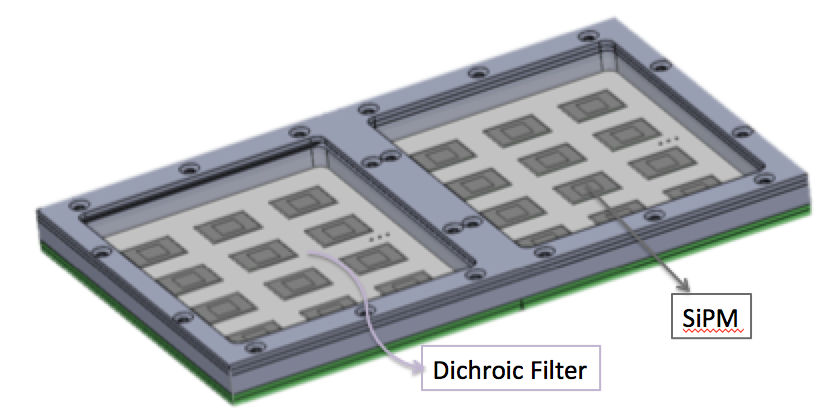
\includegraphics[height=5cm]{pds-arapuca}
%	\caption{Drawing of two ARAPUCAs, each one read-out by 12 SiPMs. This design was used for the protoDUNE.} 
%    \label{arpk}
%\end{center}
%\end{figure}
%***********************************************************************%
\begin{dunefigure}[Drawing of two ARAPUCAs of the design used for protoDUNE.]{fig:arpk}
{Drawing of two ARAPUCAs, each one read-out by 12 SiPMs; this design has been used for protoDUNE.} 
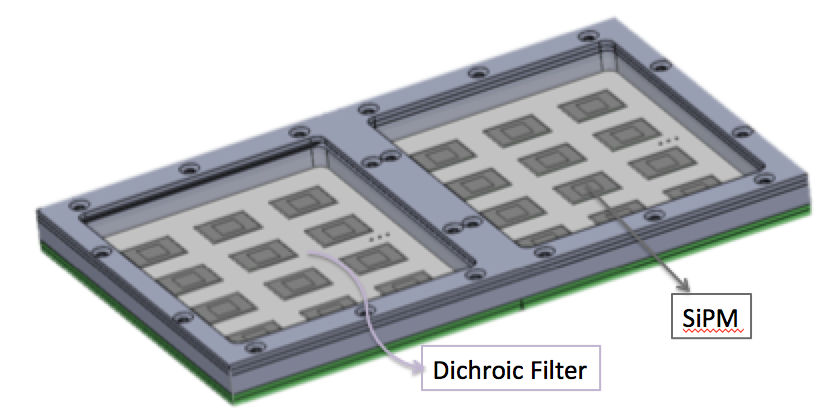
\includegraphics[height=5cm]{pds-arapuca}
%\includegraphics[width=0.8\textwidth]{image-filename}
\end{dunefigure}


{\bf The operating principle is straightforward.}

The shifters deposited on the two faces of the dichroic filter, S$_1$ and S$_2$ respectively, must have their emission wavelengths, L$_1$ and L$_2$, such that: L$_1$ $<$ L$_{cut-off}$$ <$ L$_2$, where L$_{cut-off}$ is the cut-off wavelength of the filter, that is the limit between the region of full transparency (typically $>$ 95\%) and that of full reflectivity (typically $>$ 98\%). The side of the filter deposited with S$_2$ faces the internal part of the box.

Assuming that the ARAPUCA, observes a LAr volume, scintillation VUV photons ($\lambda \sim$ 127 nm) produced by the passage of an ionizing radiation, hit the window of the device and are shifted to a wavelength of L$_1$ by the shifter deposited on the external face of the filter and enter the ARAPUCA. Once passed the filter, the photons are converted to the wavelength L$_2$ and are forced to remain trapped inside the box: its internal surface is covered with an almost perfect reflector to L$_2$ and the filter that closes the box is itself reflective to L$_2$ photons. 
Photons are trapped inside the box. After few reflections the photons are detected by the active photo-sensor installed on the internal surface of the ARAPUCA (Figure \ref{arapuca}). 

The net effect of the ARAPUCA is to amplify the active area of the SiPM used to readout the trapped photons. It is easy to show that for small values of SiPM coverage of the internal surface the amplification factor is equal to
\begin{equation}
A=\frac{1}{2(1-R)}
\end{equation}
where R is the average value of the reflectivity of the internal surfaces. For an average reflectivity of 0.95 the amplification factor is equal to ten.

%*****************************FIGURE 2*****************************%
\begin{dunefigure}[ARAPUCA and the schematic representation of the operating principle.]{fig:arapuca}
{ARAPUCA and the schematic representation of the operating principle.}
  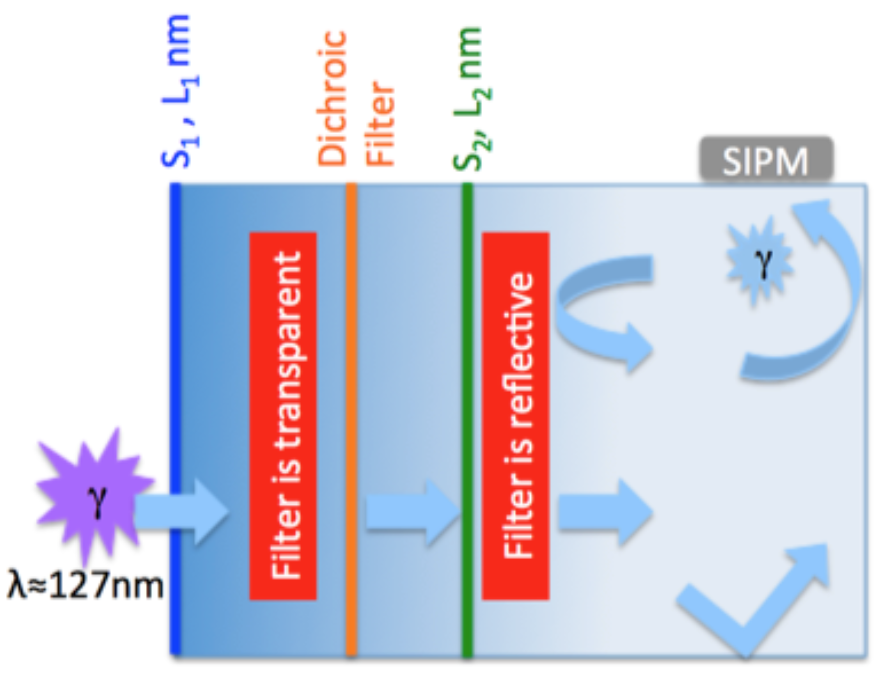
\includegraphics[height=5cm]{pds-arpkscheme}   
\end{dunefigure}
%***********************************************************************%

The next sections we describe the distinct tests of the technology at three primary locations.

\paragraph*{Tests performed in Brazil}
\label{subsec:testlnls}

Tests of the ARAPUCA in a liquid argon (LAr) environment were performed at the facilities of the Toroidal Grating Monochromator (TGM) beamline of the Brazilian Synchrotron Light Laboratory (LNLS) (Figure \ref{LNLS_test}). 

A small ARAPUCA made of PTFE with internal dimensions of 3.5x2.5x0.6 cm$^3$ was tested and a dichroic filter with dimensions of 3.5x2.5 cm$^2$ and cut-off at 400 nm was used as the window of the device.
The filter was evaporated with p-TerPhnyl (pTP), which absorbs 127 nm photons and reemits them around 350 nm,  on the external side and TetraPhnyl-Butadiene (TPB) on the internal side, which absorbs the shifted 350 nm photons and reemits around 430 nm. Trapped light was detected by a single 0.6x0.6cm$^2$  SensL SiPMs mod C60035.
The device was installed inside a vacuum tight stainless-steel cylinder closed by two CF100 flanges. The cylinder was deployed inside a LAr open bath, vacuum pumped down to a pressure around  10$^{-6}$ mbar and then filled with one liter of ultra pure liquid argon. 

LAr scintillation light emission was produced by an alpha source installed in front of the ARAPUCA, immersed in liquid argon. Signals were read-out through an Aquiris PCI board and stored on a computer.

%*****************************FIGURE 3*****************************%
\begin{dunefigure}[ARAPUCA test at LNLS]{LNLS_test}
{ARAPUCA test at LNLS} 
	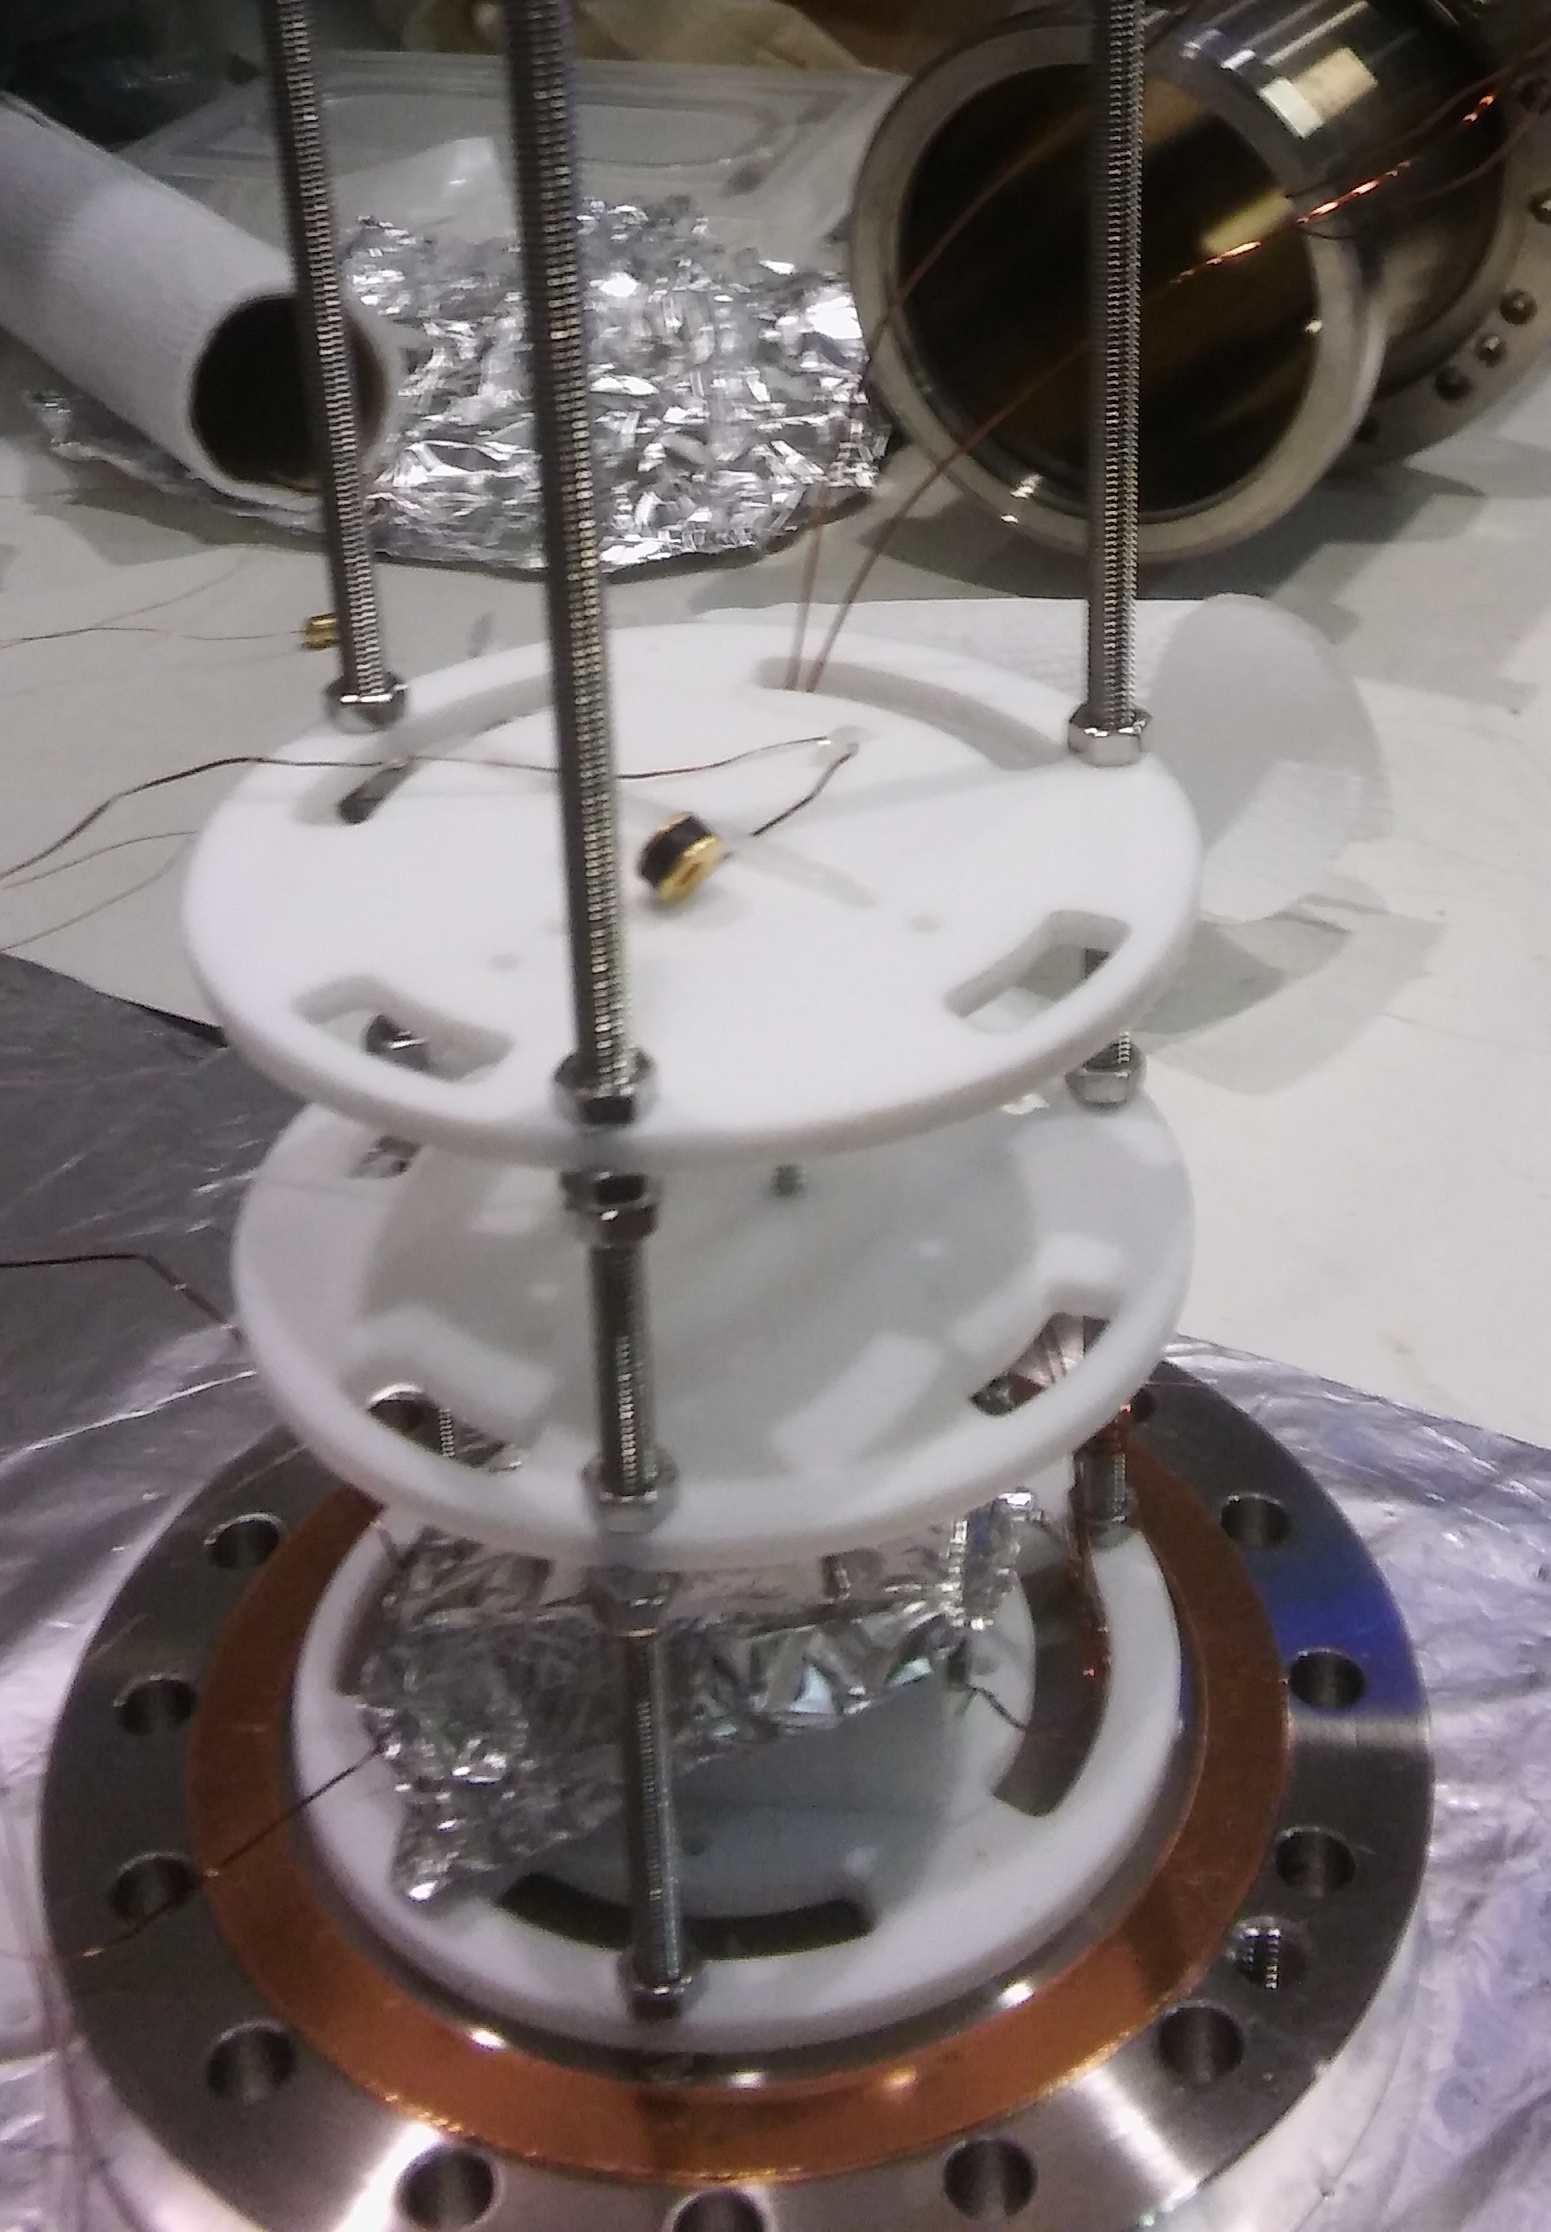
\includegraphics[height=5cm]{pds-TGM_1} \quad
	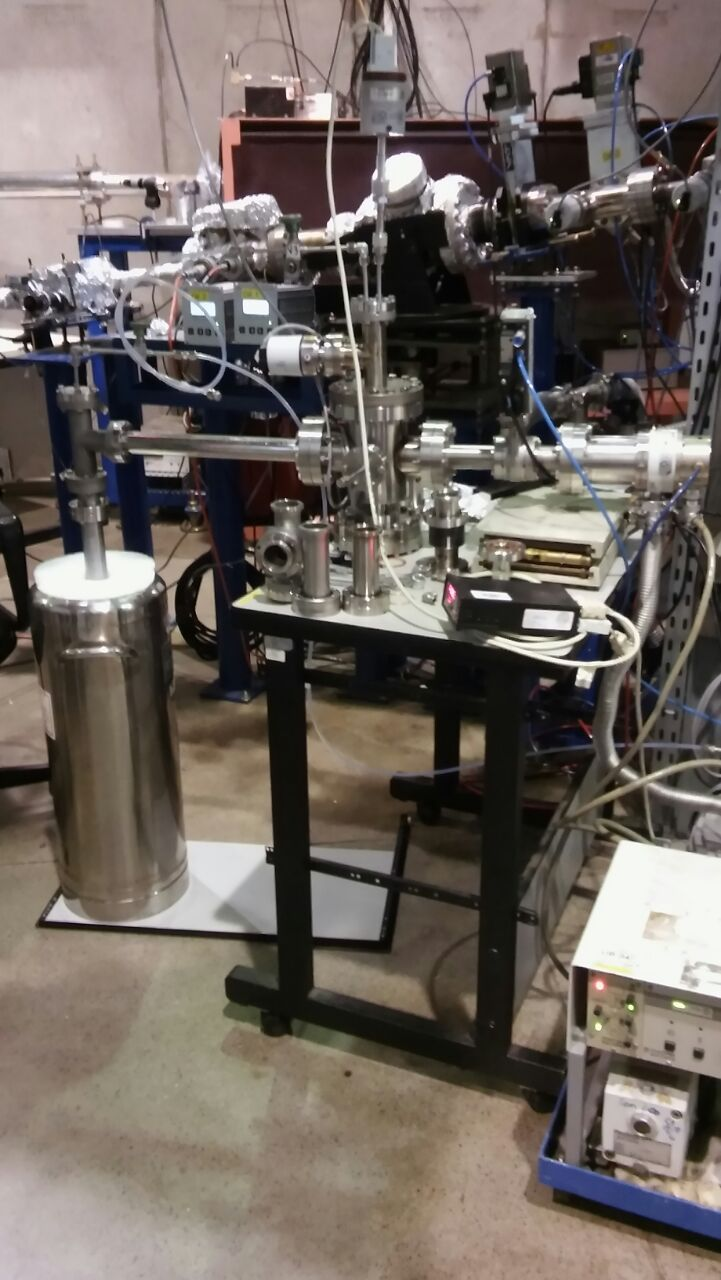
\includegraphics[height=5cm]{pds-TGM_30}\quad
	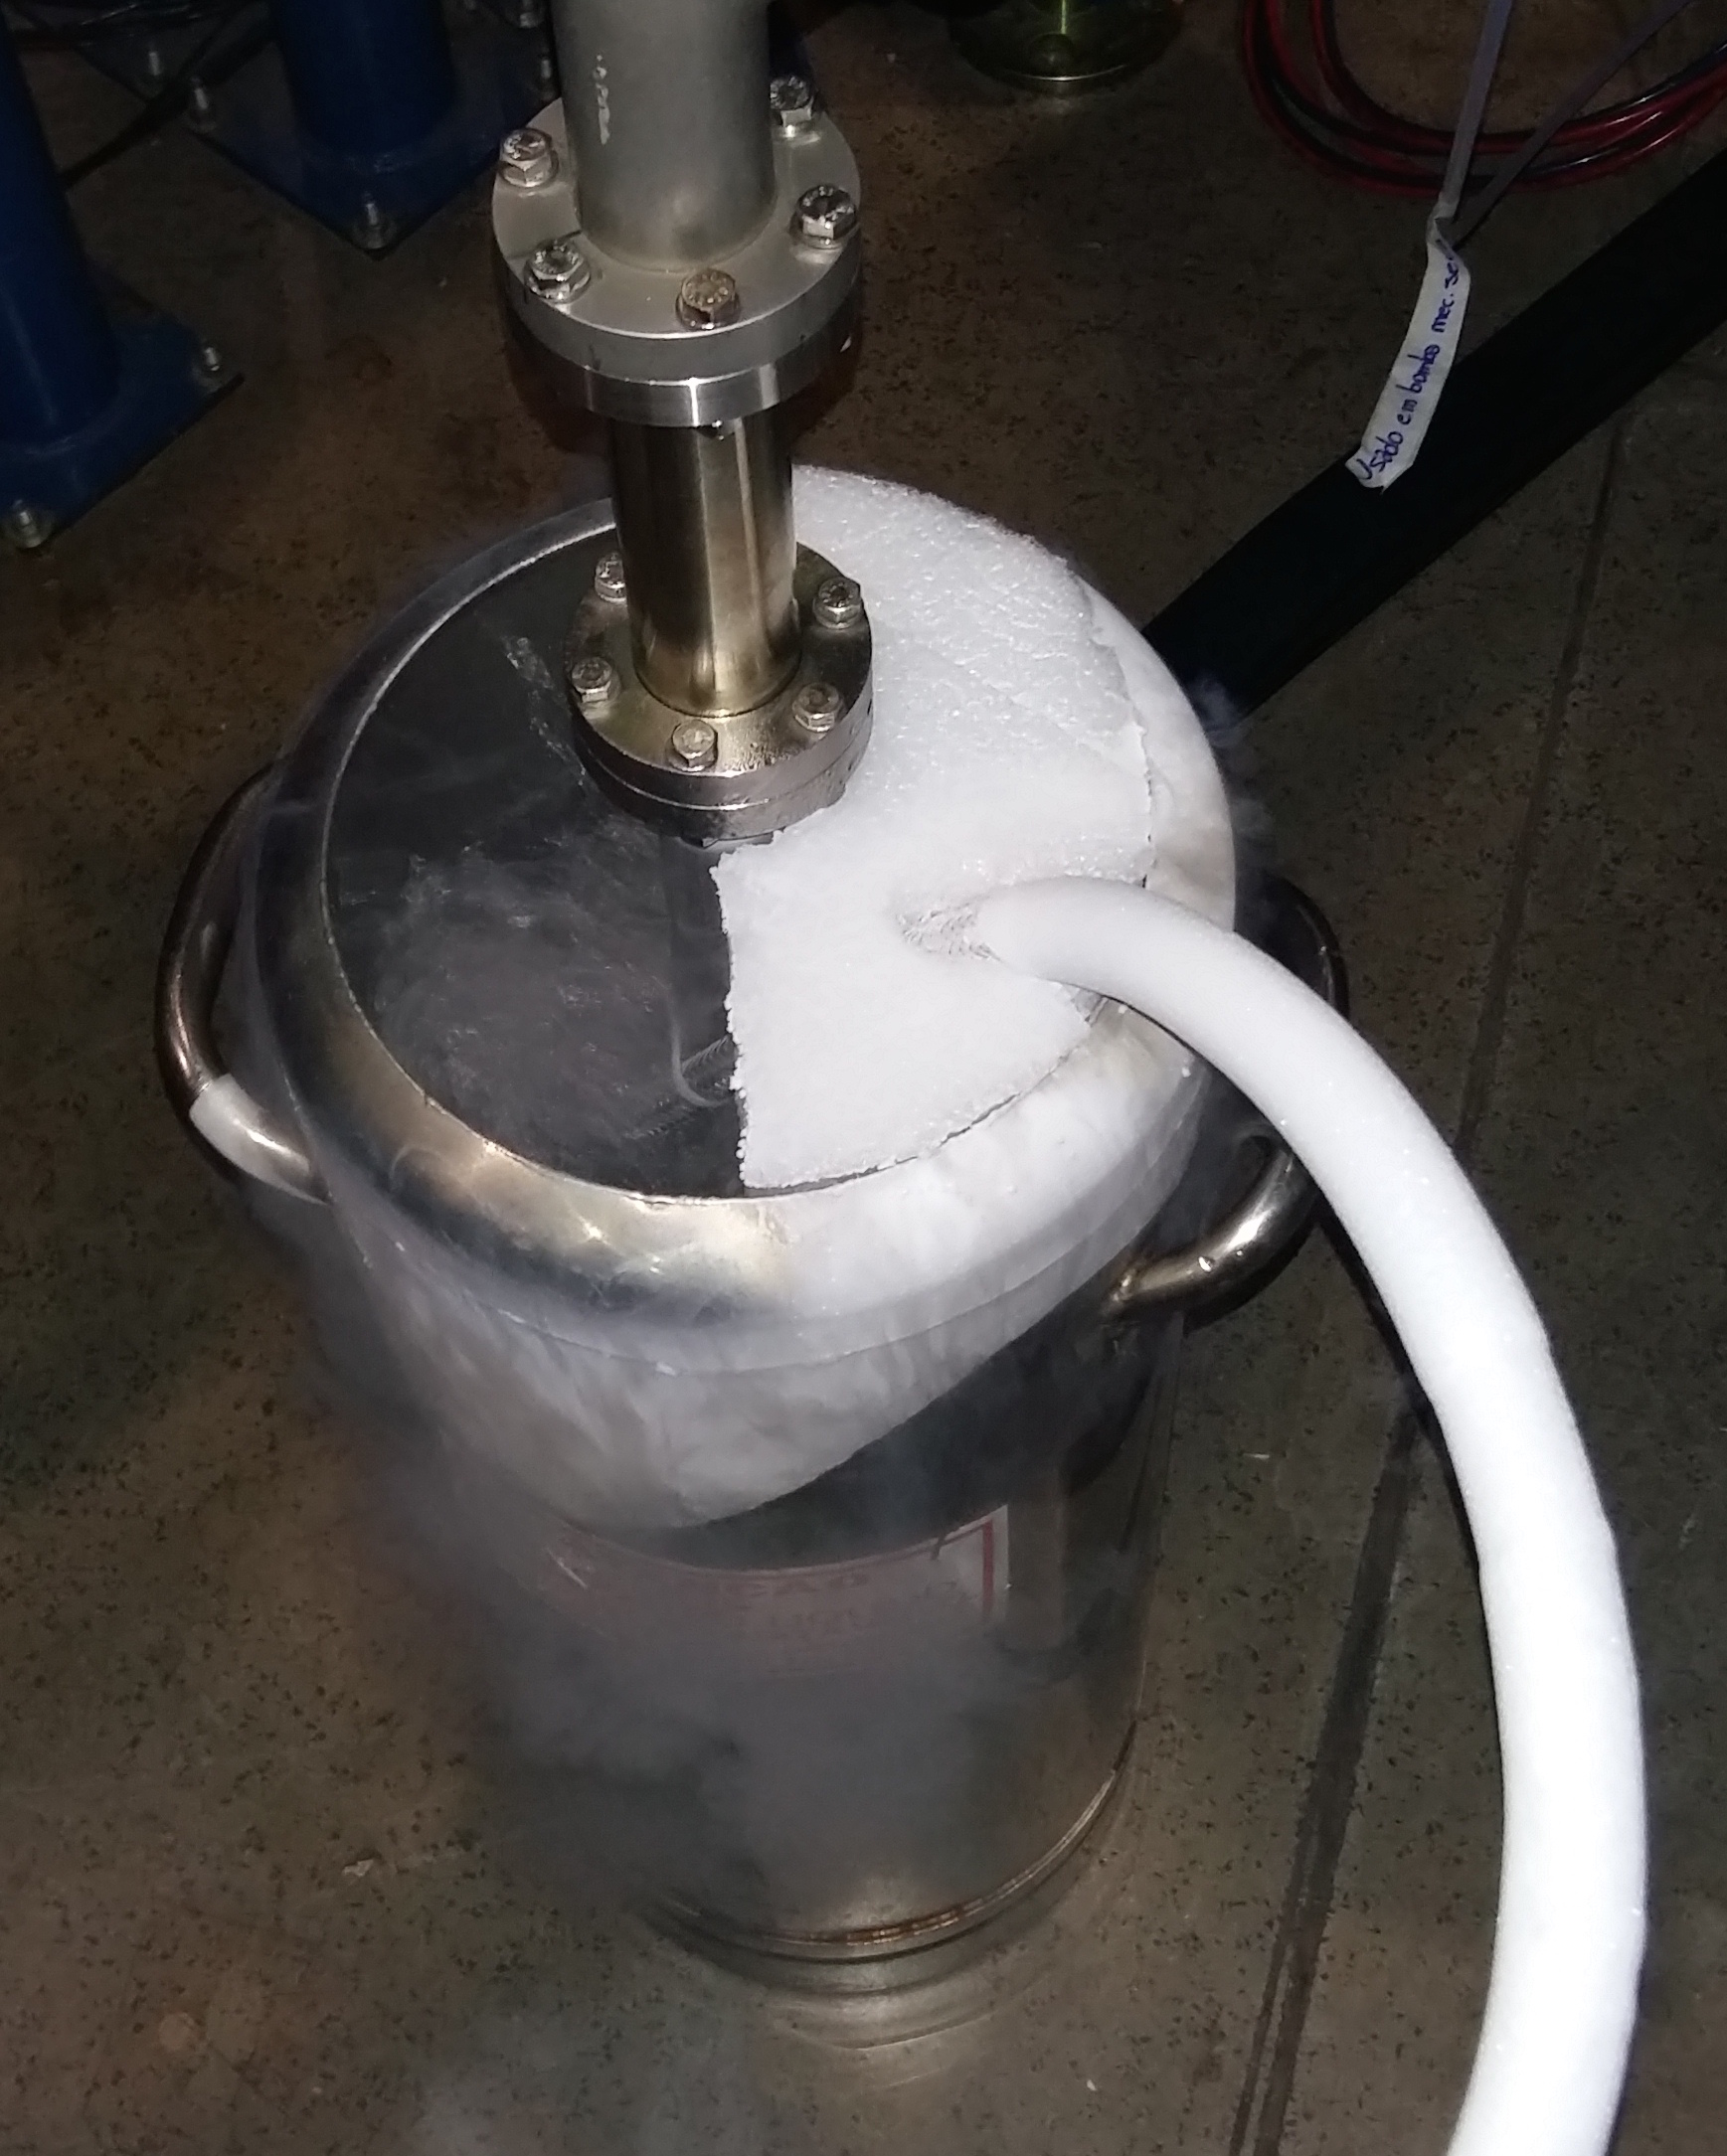
\includegraphics[height=5cm]{pds-TGM_0}
\end{dunefigure}
%***********************************************************************%

It was possible to estimate the detection efficiency of the ARAPUCA by 
determining the number of photo-electrons detected in correspondance of the end point of the $\alpha$ spectrum 
and comparing it with the expected number of photons impinging on the acceptance window for that 
particular energy value ($\sim$ 4.3 MeV), which depends only on known properties of LAr and on the solid 
anlge subtended by the the ARAPUCA window. A detection efficiency at the level of 1.8 \% 
was found, well consistent with Monte Carlo expectations.

\paragraph*{Tests performed at FERMILAB}
\label{subsec:test_fnal}

Three cryogenic tests have been performed at Fermilab up to now:
\begin{itemize}
\item the first one was performed in mid-2016 at the Proton Assembly Building (PAB) and the SCENE facility was used. The ARAPUCA prototype had dimensions of  $5.0 \times 5.0 \times 1.0$ cm$^3$ with a dichroic window of $5.0 \times 5.0$ cm$^2$ deposited with pTP and TPB, respectively on the internal and external faces. The cut-off of the filter was at 400 nm. Two SensL SiPMs mod C60035 ($0.6 \times 0.6$ cm$^2$ active area each) were installed inside the box to detect trapped photons. The ARAPUCA was deployed inside a vacuum tight cryostat filled with ultrapure LAr. An $^{241}$Am alpha source was positioned in front of the window of the device at a distance of 5 cm from its center. The efficiency of the ARAPUCA was estimated taking into account that in this case the alpha particles have a  
monochromatic energy of about 5.4 MeV. The estimated efficiency in this case was of the order of 1 \%, a factor two below what expected due to the sub-optimal quality and uniformity of the pTP and TPB films and to the lack of reflectivity of the inner PTFE surfaces;

\item the second one was performed at the beginning of 2017 at the PAB, but using a different facility, 
TallBo, which allowed to test several devices at a time. Eight different ARAPUCAs, with different 
filters (different producers), different reflectors and different dimensions where tested. The ARAPUCAs 
were exposed to the 127 nm scintillation light produced by alpha particles emitted by an $^{241}$Am 
source, mounted on a holder which could be moved with an external manipulator in order to place it in 
front of each prototype. The efficiencies of the installed ARAPUCAs ranged from 0.4 \% to 1.0 \%.

\item a third test ws performed at the end of 2017 with an array of eight ARAPUCAs together with two 
guiding bars (double-shift design) in the TallBo set-up. Data analysis is still ongoing. 

\end{itemize}

\paragraph*{ARAPUCA in protoDUNE}

Two arrays of ARAPUCAs are going to be installed inside protoDUNE to test the devices in a real experimental environment and to directly compare their performances with those of the guiding bars. The first array has been already installed in the APA 3, while the second one will be installed in the APA number 4.
 
Each ARAPUCA arrays is composed by sixteen basic cells. Each cell has the dimensions of 8 cm $\times$ 10 cm and is 
observed by 12 SiPMs (or 6 SIPMs) installed on the bottom side of the cell (6 mm $\times$ 6 mm each) and which are passively ganged together, so that only one read-out channel is needed for each 
ARAPUCA (16 channels per array). The ARAPUCA array has total dimensions of approximately 8 cm $\times$ 200 cm, exactly the same of a shifting/guiding bar. The first ARAPUCA array installed in protoDUNE is shown in figure (Figure~\ref{fig:arapuca_array}).

%*****************************FIGURE 4*****************************%
\begin{dunefigure}[ARAPUCA array in protoDUNE.]{fig:arapuca_array}
{ARAPUCA array in protoDUNE.} 	
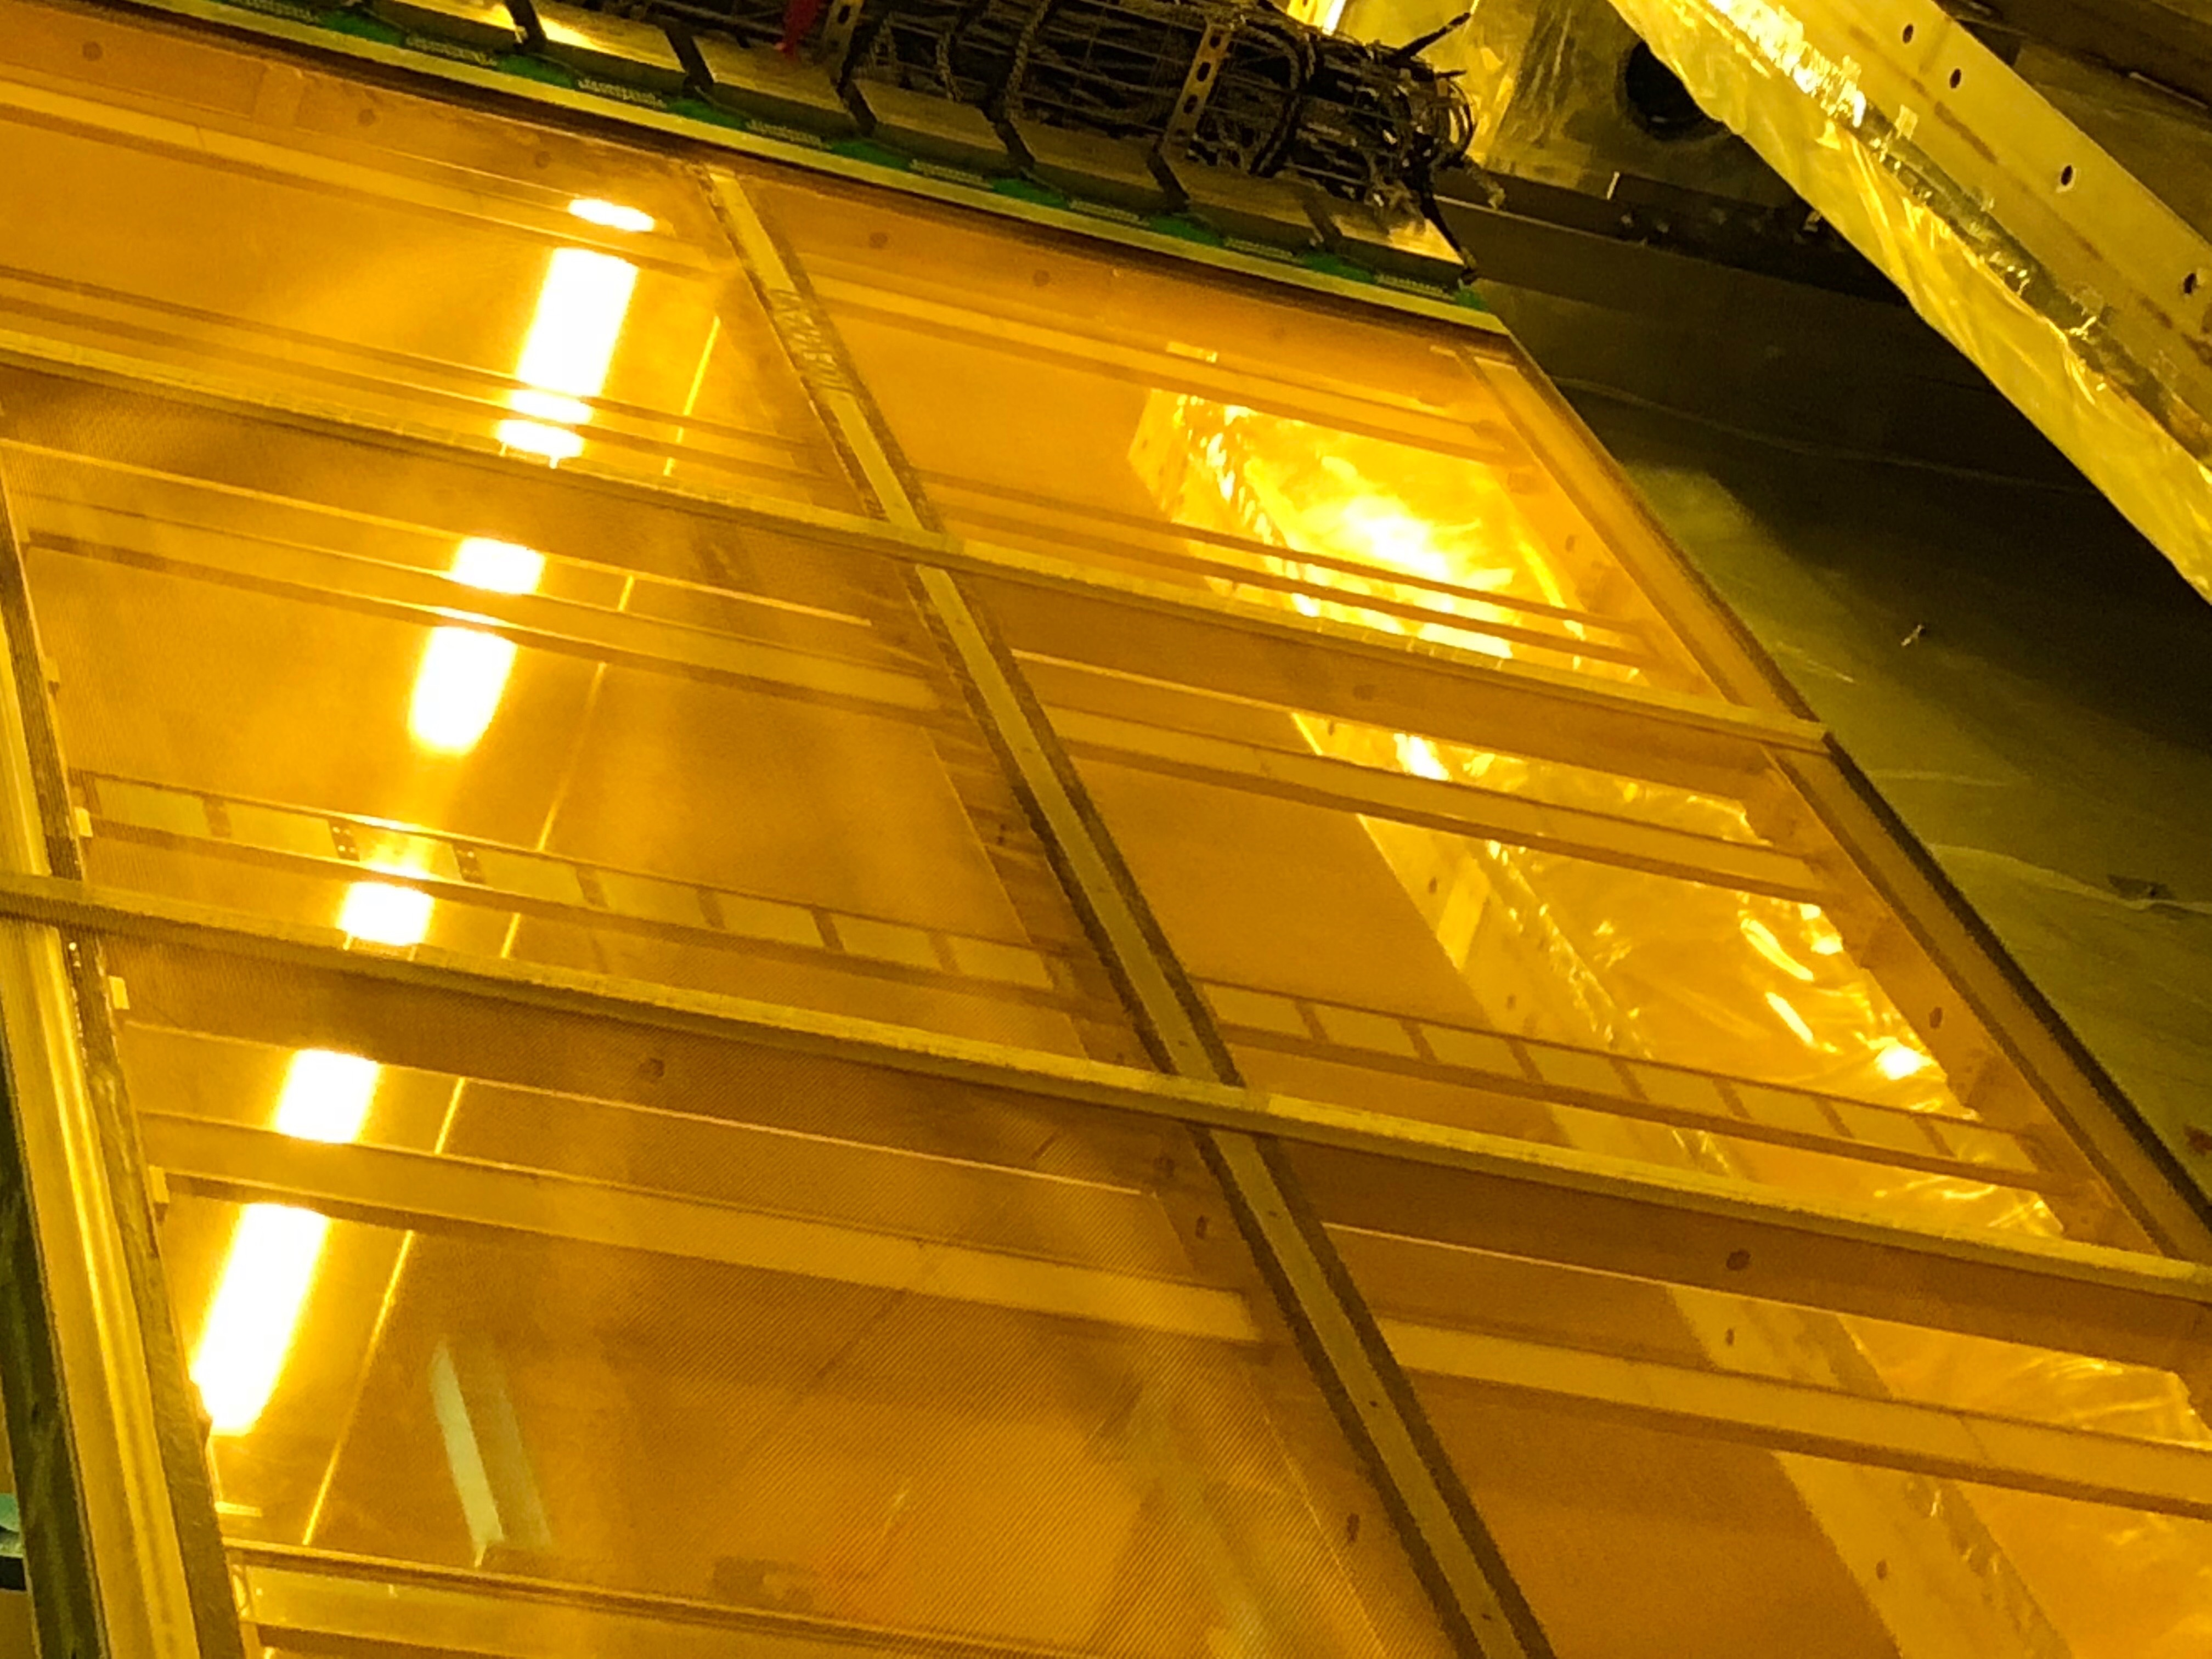
\includegraphics[height=5cm]{pds-arpkAPA3_pD.JPG} 
\end{dunefigure}
%***********************************************************************%
%\newpage

\paragraph*{Last Considerations}

The ARAPUCA device is undergoing a strong R\&D program which aims to establish its 
viability as the photon detection system of the single phase DUNE far detector, both 
in terms of absolute detection efficiency and long term reliability. Since this is a 
new technology, a strong effort needs to be put in this program in order to reach a 
full comprehension of the optical processes which are active in the device and reach 
the target efficiency of few per cent.


%\subsubsection{Hybrid or New Options (2 pages)}
%\label{ssec:fdsp-pd-pc-new}

\subsection{New Techniques to Supplement or Enhance Light Yield}
\label{sec:fdsp-pd-enh}
%\metainfo{\color{blue} Content: Cavanna/Whittington/Machado}

\subsubsection{Light Concentrators}
\label{sec:fdsp-pd-assy-lc}
%\todo{\color{blue} Content: Cavanna}
	
In the current baseline layout, the photosensitive area of the PD system is limited to about 12.5\% of the area of the anode plane - delimiting one side of the LArTPC volume. 
Only a small fraction of the VUV direct light emitted in ionization events is thus intercepted by the photosensitive area, and this fraction also quickly reduces at increasing distance of the event from the anode plane. 

Methods to increase the amount of light collected by the PDS are being considered, for example by covering the opposite cathode plane with wls-coated reflector foils so that a good fraction of the VUV light is shifted into the Visible, reflected back toward the Anode plane and eventually intercepted by the PDS, if sensitive to this wavelength.

Further increase in light collection, both for the VUV and the reflected Vis component, can be achieved by implementing large area reflective surfaces at the anode plane (e.g. in the large open areas between PD bars inside the APA frames) acting as light concentrators toward the smaller photosensitive surfaces.  
This conceptual solution is suggested from the widely diffused implementation of Winston Cones for enhancing light collection in large volume liquid detectors. 
The PD bar geometry of the photosensitive area inside the thin APA frames and the related mechanical constraints impose rather severe limitations on the design - cone depth and entrance$/$exit apertures ratio - of the light concentrating surfaces. The installation of the reflective surfaces inside the APA frame would necessarily be made before wire winding. 
Ongoing studies are expected to demonstrate the feasibility of the solution and move the conceptual scheme into a technical design. MC simulations will determine the efficiency of the light concentrator. 


\subsubsection{Hybrid and New Options}

\paragraph*{X-ARAPUCA}  X-ARAPUCA represents the main line of development of the ARAPUCA photo-detector design aiming to further improve the collection efficiency, while retaining the same working
 principle, mechanical design and active  photo-sensitive coverage.
 
In a sense X-ARAPUCA is a hybrid solution between the ARAPUCA and the wavelength-shifting light guide bar PDS concepts, 
where photons trapped in the ARAPUCA box are shifted and transported to the readout via total internal reflection in a light guide placed inside the box.
This solution minimizes the number of reflections on the internal surfaces of the box and thus the probability of photon loss. Simulations suggest that this modification will lead to a rather significant increase of the collection efficiency.

 \begin{dunefigure}[X-ARAPUCA design (exploded view).]{fig:exploded}
{X-ARAPUCA design (exploded view).}
 % \vspace{-2.5cm}
   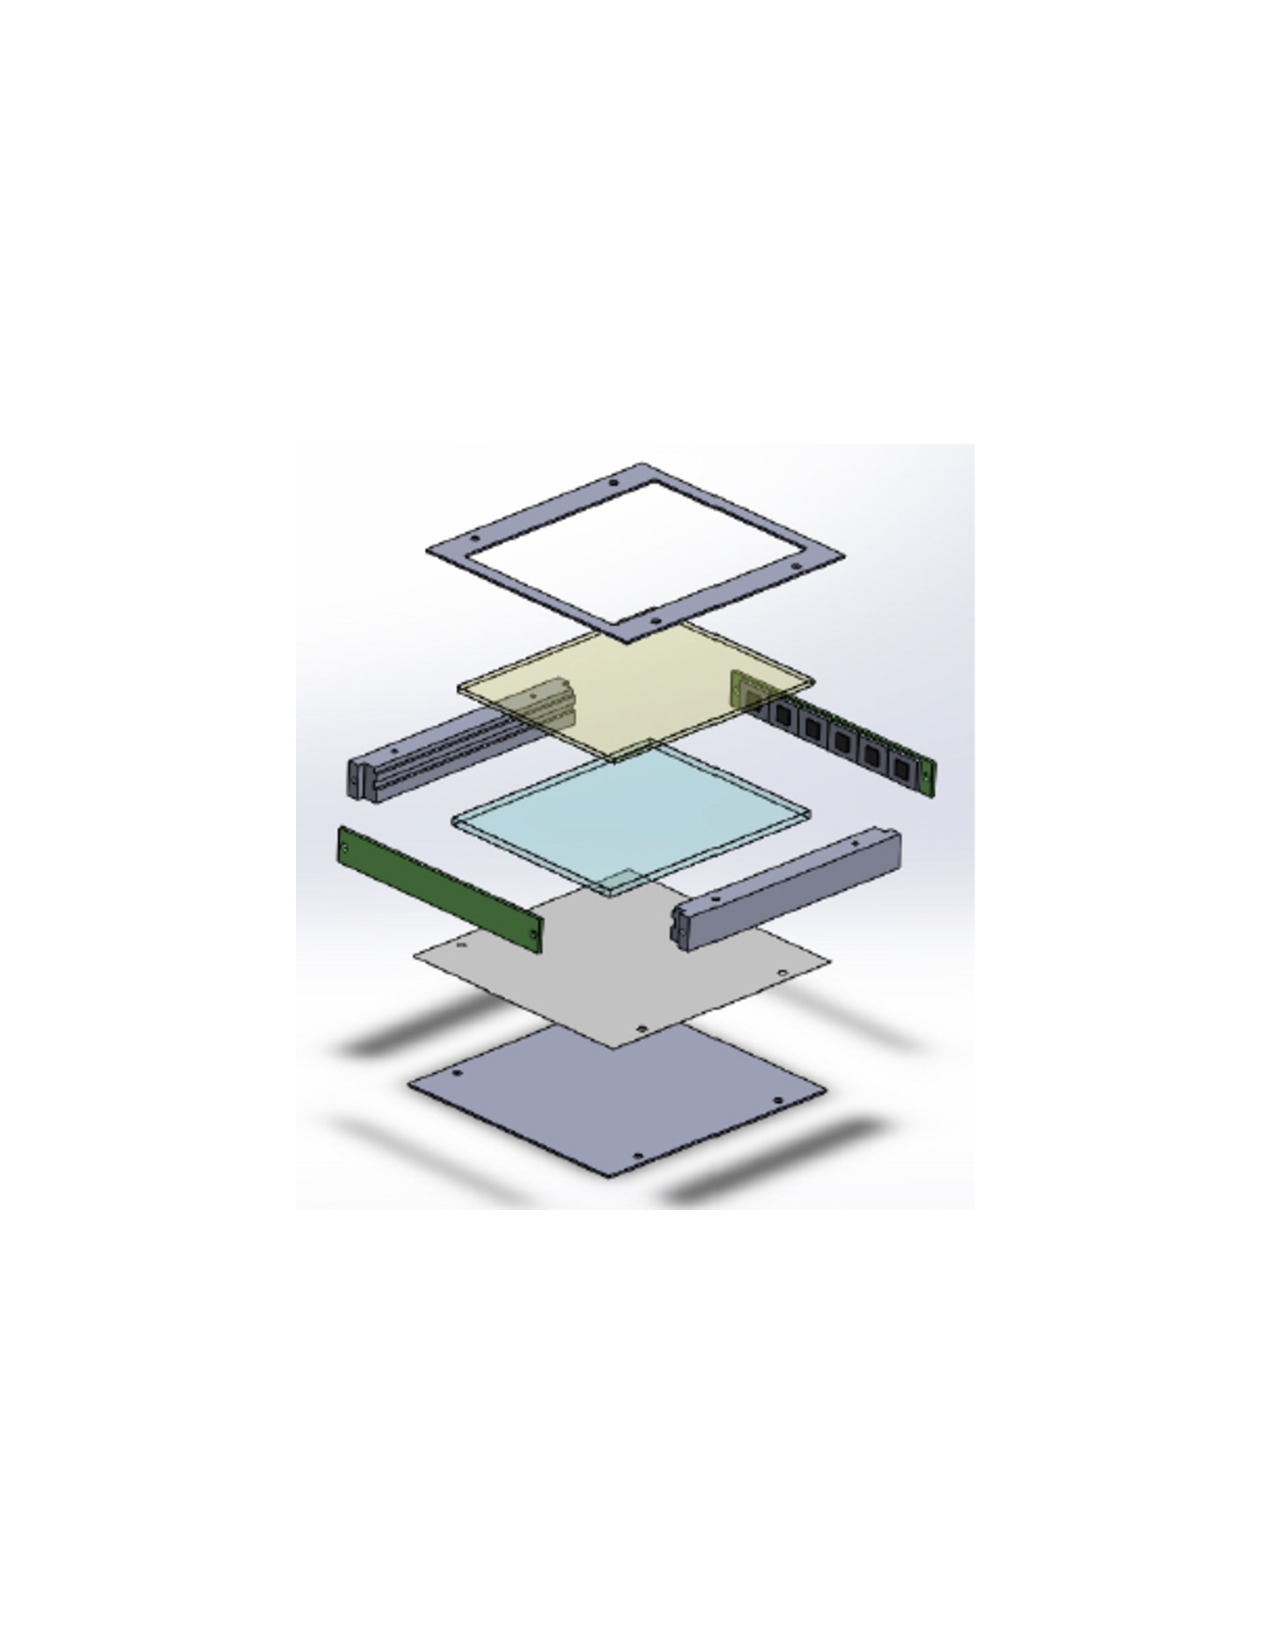
\includegraphics[height=.5\textheight]{pds-X-Arapuca-exploded-view.pdf}
\end{dunefigure}

 In a standard ARAPUCA the photon trapping effect is obtained by means of a dichroic filter and a two-steps wavelength shifting process, the first from VUV to UV outside the acceptance window of the box and the second inside from UV to blue, across the filter cutoff. Double shifted photons are eventually collected by an array of photosensors (SiPM) distributed on the backplane of the box, opposite to the the acceptance window. In the X-ARAPUCA design, Figure \ref{fig:exploded}, the inner shifter coating/lining over the reflective walls of the box is replaced by a thin wavelength-shifting light guide slab inside the box, of the same dimensions of the acceptance filter window and parallel to it. The SiPM arrays are installed vertically on the sides of the box, in optical contact to the light guide thin ends. 
 In this way a fraction of the photons will be converted inside the slab and guided to the read-out, other photons,  e.g. those at small angle of incidence below the critical angle of the light guide slab, after conversion at the slab surface will be remain trapped in the box and eventually collected as for the standard ARAPUCA.
 
 A full sized X-ARAPUCA prototype is under construction. The light guide is made by a 2 mm thick TPB doped acrylic slab. Specially designed read-out boards have been realized, made of 6 passively ganged SiPMs in a strip configuration.  Two boards into a single channel readout light signals from the X-ARAPUCA box. 
 
 The photon detectors described in the preceding section represent the results of a long process of optimization of the initial concepts developed years ago. A balance between the cost of the readout electronics (channel count), and the cost and performance of the SiPM's was achieved with realistic designs of the photon detectors offering the detection efficiency in the range $\sim$ 0.5 to 1.5\%.
 
A significant advances in the technology of the SPM's have been accomplished during this time: the photosensors dark count, after-pulsing and cross-talk rates have been lowered by almost an order of magnitude, whereas the production costs have been dropping significantly in response to the increasing range of applications.  The recent studies and tests demonstrate that the improved quality of the photodetectors is permitting much higher degree of ganging (passive or active), thus significantly lowering the ``per SiPM" readout costs.
These technological trends are likely to continue, thus allowing for a possible alternative concepts of the Photon Detectors, even within the geometrical and cost confines of the baseline detectors.\\
One of the possible different concepts of the Photon Detector includes a long printed circuit board with the overall dimensions identical to the light guide bars or ARAPUCA but with a simpler construction involving only SiPMs distributed over the board surface. The SiPMs can be coated with  appropriate waveshifter (TPB or MSB) or a foil with the waveshifter in front of the SiPM can be used to convert the VUV 128 nm Argon light to the blue light at the maximum detection efficiency of the SiPM. The overall detection efficiency of such a ``detector element"is expected to be of the order of 25-30\%, depending on the pixel size and the fill-factor of the SiPM.

A photon detector involving the SiPMs only would offer a major simplification of the construction and integration efforts. Its overall performance can be reliably estimated and it is proportional to the total area of the bar covered with the SiPMs.
The performance of the baseline Photon Detectors can be achieved with 2-4\% of the area covered with the SiPMs. Taking 1800 cm$^2$ as a bar surface this coverage can be accomplished with 100-200 SiPMs of the standard 6x6 mm form factor. With 12-fold passive ganging, successfully demonstrated in recent tests, such a solution would require 8-16 readout channels per bar. The multiplexing level is limited by the noise of the readout electronics. Significantly higher degree of multiplexing can be achieved by use of larger pixel (like 75x75 microns) SiPMs and/or possible cold active ganging circuitry. 
Such a detector concept appears very flexible and it would allows for future optimization in response to the expected technological advances with no or minimal impact on the rest of the DUNE  detector. 


\paragraph*{Beyond the TDR} The Technical Proposal and TDR may include proposals to augment the capabilities of the photon
collector modules. In the case that the hardware requirements for such proposals would pose a minimal
impact on the detector design, additional R\&D beyond the timescale of the TDR may be required since it may impact the second 10~kt module if not the first. 
Some examples include:
\begin{itemize}
\item TPB-Coated Reflector Foils %(Szelc)
\item Xenon-Doped LAr %(Escobar/Para)
\item TPB-Doped LAr %(Escobar)
\end{itemize}

%%%%%%%%%%%%%%%%%%%%%%%%%%%%%%%%%%%

\subsection{Photon Sensors}
\label{sec:fdsp-pd-ps}
%\todo{\color{blue} Content: Zutshi}

The SP DUNE Photon Detector System will use Silicon Photomultipliers, mated to
the bar or ARAPUCA photon collector options, to detect scintillation light generated in the LAr. Robust photon detection efficiency, low operating voltages, small size and ruggedness make their usage entirely plausible in the single
phase design where the photon detectors are to be accommodated inside the APA 
frames. The salient guiding principles of this SiPM-based photo-detection system can be stated
as:

Signal path separate from TPC readout. This implies cables dedicated to bringing the power
in and taking the analog or digitized signals from the PD system, out of the cryostat. 
Feed-through cable space limitations therefore, imply some level of ganging of the SiPM
signals inside the LAr volume. 

The optimal SiPM may depend on the photon collector option. Since all photon collector
options being currently considered involve shifting the 128 nm LAr scintillation to 
varying degrees, the final fine-tuned choice may have to be made after the collector
down-select. It should however be kept in mind that the size of these effects, while not 
anything to sniff at, will not exceed 15-20 $\%$.

The Silicon Photomultiplier packaging should allow for tileable arrays to be constructed to
facilitate high efficiency mating to the photon collectors and efficient space utilization inside
the APA frame.

While understanding SiPM requirements (number of devices, dynamic range, triggering, 
zero-suppression threshold etc.) in light of the physics goals is an ongoing process, it is clear
from the R$\&$D carried out so far that devices from a number of vendors have the 
performance characteristics in the vicinity of that needed for the DUNE photon detector
system (see Table xxx). Furthermore, a number and types of these devices are being installed in 
protoDUNE which will provide an excellent test bed for evaluating and monitoring SiPM
performance in a realistic environment over the medium term. 

A key requirement, based on past experience, is ensuring the mechanical and electrical 
integrity of these devices in a cryogenic environment. This is a DUNE requirement which 
catalog devices from most vendors do not satisfy as they are only certified for operation 
down to -40$^\circ$C. Thus it is of paramount importance for the DUNE PD Consortium to work 
with vendors in designing, fabricating and certifying SiPM packaging that is robust and
reliable from the point-of-view of long-term operation in a cryogenic environment. Already 
there is interest from at least two vendors (Hamamatsu and FBK) to engage with the
Consortium in this fashion with the goal of having the vendor warrantying the product
for our application. Contact with other vendors and experiments (e.g. DarkSide) is
being pursued.   

In parallel, comparative performance evaluation of promising SiPM candidates from
multiple vendors will need to be carried out. This evaluation will not only need to
address inherent characteristics (gain, dark rate, x-talk, after-pulsing etc) and ganging 
performance but also form factor, spectral response and mating with regard to the
multiple photon collector options. Experience acquired from protoDUNE construction
and operation will inform QA/QC plans for the full detector which will need to be
delineated in detail.

%%%%%%%%%%%%%%%%%%%%%%%%%%
%The planned photodetector is a SiPM, model 
%SensL C-Series 6~mm$^2$
%(MicroFB-60035-SMT). % device. 
%This model of SiPM has a detection efficiency of
%41\%; the quoted detection efficiency incorporates Quantum Efficiency (QE) and 
%the effective area
%  coverage accounting for dead space between pixels.   At LAr temperature (89~K) the dark rate is of order 10~Hz
%(0.5 p.e. threshold), and  after-pulsing has not been observed. An on-going testing program is in place to ensure 
%that the SiPMs can reliably survive the stresses associated with 
%any thermal cycling in LAr and long-term operation at LAr temperature.

%All photodetectors %for ProtoDUNE-SP 
%are subjected to testing to determine
 %forward and reverse bias I-V curves,
 %breakdown voltage, dark current and dark count rate, photodetector gain, crosstalk estimation, response, and bias dependence of parameters.
 
%All SiPMs 
%Each SiPM is tested before mounting on the readout boards to determine
%if the part meets the specifications in a warm test.  After mounting to
%the readout board all items are tested both warm and cold (cyrogenic 
%temperature) to determine the operating characteristics.

%In addition to these tests, the photodetectors are tested for their
%response to light signals from an LED of appropriate wavelength.
%These tests will be sensitive enough to determine if one of the three SiPM
%elements operating in parallel is not functioning.


%%%%%%%%%%%%%%%%%%%%%%%%%%%%%%%%%%%
\subsection{Electronics}
\label{sec:fdsp-pd-pde}
%\metainfo{\color{red}\bf  Content: (3 pages) - Moreno/Franchi/Djurcic}
%\todo{\color{blue}  Content: Moreno/Franchi/Djurcic}

Scintillation light from LAr comes from two different excited states with lifetimes of about 6 ns and 1.6 $\mu$s.
Only a limited amount of light is collected, so the electronics are designed to collect the light from both excited states. A summary of the general requirements for the system, including initial requirements from a physics performance perspective, are given in Table~\ref{tab:fee_req}.
%
\begin{dunetable}[Physics requirements for the PDS electronics]{ll}{fee_req}{Physics requirements for the PDS electronics}
 Performance Parameter       & Target   \\ \toprowrule
Time Resolution                   & Better than 30 ns wrt event time zero (``t0'')      \\ \colhline
 Charge Resolution               & 0.25 photo-electron equivalent                    \\ \colhline
 Dynamic Range                   & $\sim \times$10 better than detector (1000:1)         \\ \colhline
 Linearity                               & Sufficient to resolve 1 photo-electron signals   \\ \colhline
 Multi-Hit Capability              & Sufficient to measure Triplet (late) Photons          \\ \colhline
 Dead Time                           & Live up to 2 drift times either side of beam spill         \\ \colhline
 Bias Control                        & 0.1 V resolution up to 30 V per channel  \\ \colhline
 Calibration                          & On-board Charge Injection  \\ \colhline
 Timing                                 & Events time-stamped via ProtoDUNE Timing System  \\    \end{dunetable}

Electronic design definition need to be based on R\&D activities to meet the physics requirements. An important aspect to be determined is the type of data to be processed.
In general arrival time and total charge are the parameters to be obtained from a detector. Evaluation of these parameters is possible using analog or digital system. 
Charge preamplifier is connected to the output of the detector to integrate current producing a charge proportional output. In the case of digital systems an amplifier is needed to adjust the detector output signal level to the input of an Analog to Digital Converter.  In both systems, characteristics like sampling rate, number of bits, power requirements, signal to noise ratio among other should be evaluated to arrive to a final solution.  Pulse shapes can be fully analyzed to improve detection of  SNB but it will have an important impact on the readout scheme and the digitalization frequency.

Photon sensors ganging scheme, closely related with the type of signal to be processed, have a direct impact on the localization of the electronic components. In the case of active ganging (sensors connected in series), amplifiers and ADCs need to be placed very close to the detectors, inside the LAr volume, bringing into play characteristics to be addressed like the time stability of the components in cold environment, power dissipation, among others. In the case of passive ganging, analog signals are transmitted outside of the cryostat for processing and digitalization. 

A close interface with photo sensor groups, physics and simulations is required to address the aforementioned issues. As mentioned R\&D activities need to be conducted  previous TDR to meet some requirements of the readout electronics. ProtoDUNE operation is another valued information source. In following a summary of the electronic readout scheme implemented in protoDUNE is given.

\begin{dunefigure}[Block diagram of the protoDUNE SSP module]{PD_fig-e-3}{Block diagram of the protoDUNE SSP module} 
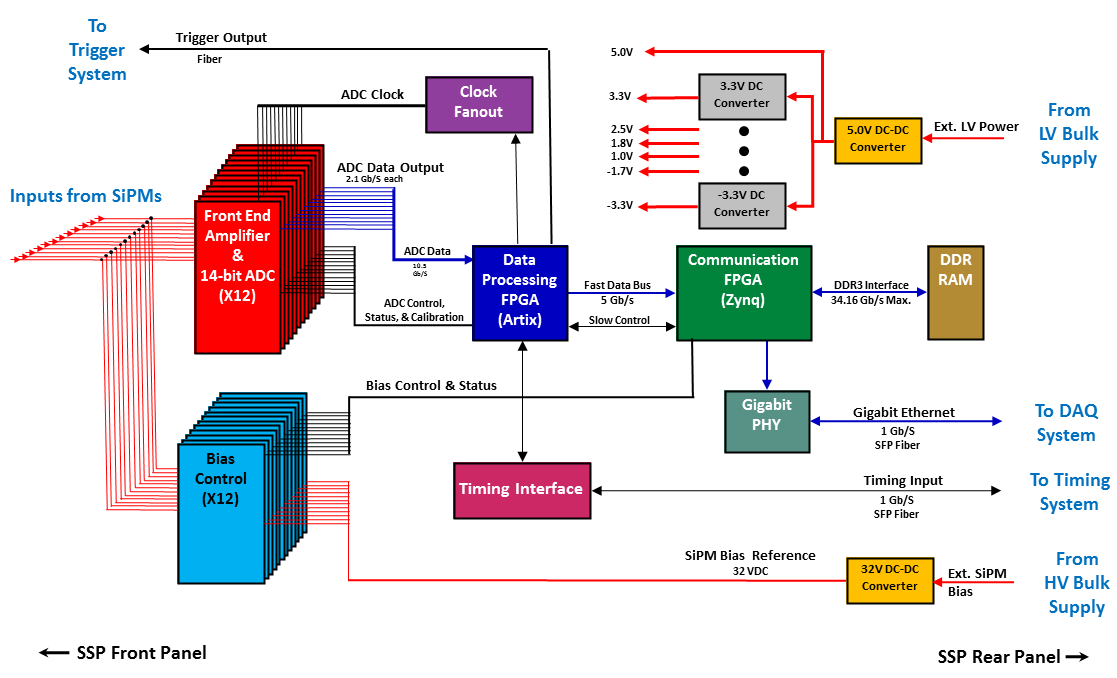
\includegraphics[width=\textwidth]{pds-ProtoDUNE-SSP-block-diagram.png}
\end{dunefigure}

Independent cables are used in protoDUNE for the TPC electronics and PD electronics. That situations impose a limit in the number of cables to bring the signal outside the cryostat.  A passive ganging scheme was chosen, where three SiPMs are ganged together.  
The unamplified analog signals from the SiPMs are transmitted directly to outside the cryostat
for processing and digitization, with the advantage that the infrastructure required for inside the cryostat is  
reduced (power, data cables, precision clocks, data protocols). Therefor there is not PDS front-end electronics in the LAr cold volume. 
A custom module, called the SiPM Signal Processor (SSP), receives the SiPM signals outside the cryostat. An SSP consists of 12 readout channels packaged in a self-contained 1U module.  

%
Each channel contains a fully-differential voltage amplifier and a 14-bit, 150-MSPS analog-to-digital converter (ADC) that 
digitizes the waveforms received from the SiPMs.  
The front-end amplifier is configured as fully-differential, and receives the SiPM signals into a termination resistor that 
matches the characteristic impedance of the signal cable. 
Currently there is no shaping of the signal, since the SiPM response 
is slow enough relative to the speed of the digitization to obtain 
several digitized samples of the leading edge of the pulse for the determination of signal timing.  A block diagram of the system is shown in Figure~\ref{fig:PD_fig-e-3}.

%The processing is pipelined, and performed by a Xilinx Artix Field-Programmable Gate Array (FPGA).  
%The FPGA implements an independent Data Processor (DP) for each channel.  
%The processing incorporates a leading edge discriminator for detecting events
%and a constant fraction discriminator (CFD) for subclock timing resolution.  

In the standard mode of operation, the module performs waveform capture, 
using either an external or internal trigger.  
In the latter case the module self-triggers to capture only waveforms with an amplitude greater than
a specified threshold.
%on a waveform  above predetermined  threshold. 
Up to 2048 waveform samples may be read out for each event, with the current firmware 
configuration. 
%Because  the Xiling Artix FPGA  is programmable  and accessible, it is possible to  explore  
%different data processing algorithms  and  techniques,  and then  summarize
%information  on  processed  waveforms  in % terms  of  
%a header output. 
%It is also possible to customize the readout for a given type of event (e.g., a supernova).  
%When waveform readouts overlap, the device can be configured to offset, 
%truncate or completely suppress the overlapping waveform.  
%Pile-up events can also be suppressed.  A picture of the prototype module is shown in Figure%~\ref{fig:PD_fig-e-2}.  
%Fig. xx3.  Picture of the SSP module.

%In order for the events measured in the photon detector to be matched up 
%with the corresponding events in the TPC, the front-end electronics 
%attaches a timestamp to the data as it is acquired.  
%The timestamp is unique, and has a correspondence with the timestamps in 
%the TPC electronics processing.  
%The timestamp in the SSP is applied to the event data as it is digitized. 
%In the case where zero-suppression and data sparsification are used, 
%the timestamp on accepted data remains intact.  
%To achieve this, the TPC and PD electronics must be synchronized, 
%including timestamp counter resets, based on a known and stable calibration 
%for the timing resolution of the ADC conversion between the two systems.  
In the protoDUNE-SP the photon readout is configured to read waveforms when triggered by a beam event,
and/or to provide header information when self-triggered by cosmic muons.
The header portion summarizes pulse amplitude, integral, and time-stamp information of events.
%and will capture times over threshold of waveforms, and will capture the timestamp of the event. 

A Xilinx Zynq FPGA handles the slow control and event data transfer.  
The SSP for protoDUNE-SP uses Gb Ethernet communication implemented over an optical interface.
The 1 Gb/s Ethernet supports full TCP/IP protocol.  
The module includes a separate 12-bit high-voltage DAC for each channel to 
provide up to 30\,V of bias to each SiPM.  
The module also features charge injection for performing diagnostics and linearity 
monitoring, and also voltage monitoring.

%In tests to date, the SSP has been able to measure single photo-electron signals 
%coming from the SiPMs over a cable length of 25 meters, when three SiPMs 
%are summed together and operated at LAr temperatures.  
%The timing resolution of the signals has been measured to be better than 3\,ns.  
%The full-differential signal processing in the front-end circuitry 
%is important in achieving this result.

The SSP provides a trigger output signal from internal discriminators in firmware based on programmable
coincidence logic, with a standard ST fiber interface to the central trigger board (CTB).
Input signals are provided to CTB from the beam instrumentation, the SSPs, and the beam TOF system.
The CTB receives timing information from the protoDUNE-SP timing system and the CTB trigger inputs are distributed to 
the experiment via the timing system.
To that end the SSP implements the timing receiver/transmitter endpoint hardware to receive trigger inputs and clock signals from the timing system.
%A block diagram of the system is shown in Figure%~\ref{fig:PD_fig-e-3}.
%
%\begin{dunefigure}[Block diagram of the ProtoDUNE SSP module]{PD_fig-e-3}{Block diagram of the ProtoDUNE SSP module} 
%\includegraphics[width=\textwidth]{ProtoDUNE-SSP-block-diagram.png}
%\end{dunefigure}

%\fixme{rjw: Include comment whether there are differences between the photon collector options}

%%%%%%%%%%%%%%%%%%%%%%%%%%%%%%%%%%%
% Combined into single QAQC section 
%\subsection{Quality Assurance}
%\label{sec:fdsp-pd-qa}
%\metainfo{\color{blue} Content: (1 page) - Warner}

